\documentclass[pdftex,a4paper]{article}
\usepackage[lmargin=1.25in,rmargin=1.25in,tmargin=1in,bmargin=1in]{geometry}
\usepackage[T1]{fontenc}
\usepackage{lmodern}
\usepackage{textgreek}
\usepackage[utf8]{inputenc}
\usepackage[czech]{babel}
\usepackage{url}
\usepackage{graphicx}
\usepackage[usenames,dvipsnames]{xcolor}
\usepackage{listings}
\usepackage{needspace}
\usepackage{mathtools}
\usepackage[unicode,pdfdisplaydoctitle,pdftex,colorlinks,allcolors=black]{hyperref}
\hypersetup {pdftitle={KIV/SU},pdfauthor={Kareš, Matěj; Kinkor, Vojtěch}}
\title{Vizualizace grafu matematické funkce}
\author{Vojtěch Kinkor}
\date{\today}


\lstset{
	backgroundcolor=\color{white},
	basicstyle=\footnotesize\ttfamily\fontfamily{pcr}\selectfont,
	breakatwhitespace=true,
	breaklines=true,
	commentstyle=\itshape\color{Gray},
	keywordstyle=\bfseries\color{blue},
	stringstyle=\color{ForestGreen},
	escapeinside={\%*}{*)},
	frame=none,
	keepspaces=true,
	numbers=none,
}


\begin{document}

\begin{titlepage}
\begin{center}


~\\[2.5cm]

\includegraphics[width=0.7\textwidth]{res/logo}
\\[0.5cm]


{ \huge \bf Semestrální práce z předmětu\\ KIV/SU \\[0.6cm] }
{ \LARGE \sc Shlukovací algoritmy }

\vfill

% Author and supervisor
\begin{minipage}{0.49\textwidth}
\begin{flushleft} 
\emph{Datum:}\\
\today
\end{flushleft}
\end{minipage}
\begin{minipage}{0.49\textwidth}
\begin{flushright} 
\emph{Vypracovali:} \\
Matěj \textsc{Kareš}\\
Vojtěch \textsc{Kinkor}
\end{flushright}
\end{minipage}



\end{center}
\end{titlepage}

\newpage
\tableofcontents
\newpage




\section{Zadání}

Cílem práce je vytvoření aplikaci pro shlukovou analýzu dat různými metodami. Aplikace bude umožňovat pracovat s daty libovolné dimenze. Součástí bude vizualizace dat ve 2D prostoru (tedy v prostoru omezeném na jednu až dvě dimenze) v podobě bodového grafu. Data bude možné náhodně vygenerovat, případně načíst ze souboru. Výsledek shlukování bude možné exportovat do souboru.




\section{Shluková analýza}

Shluková analýza (případně též shlukování, clusterová analýza, clusterizace) se zabývá postupy, pomocí kterých lze v netříděných data nalézt shluky dat s podobnými vlastnostmi. Cílem je, aby podobnost dvou objektů v jednom shluku byla maximální, zatímco podobnost objektů v různých shlucích byla minimální. Výsledkem je nalezení vztahů mezi objekty bez vysvětlení, proč tyto vztahy existují.

Shlukem tedy nazýváme skupinu objektů, které jsou si navzájem podobné a rozdílné od objektů z jiných shluků.

Obvykle se mluví o tzv. \uv{hard} shlukování, které znamená, že shluky jsou vzájemně disjunktní a každý objekt patří právě do jednoho. V opačném případě se jedná o \uv{soft} nebo fuzzy shlukování — každý objekt může patřit do více shluků zároveň.

V rámci strojového učení se jedná o metodu učení bez učitele (unsupervised learning).

Shluková analýza má mnohé uplatnění, mj.:
\begin{itemize}
	\item při porozumění datům a jejich struktuře
	\item použití v biologii (např. seskupení DNA sekvencí do genových rodin)
	\item průzkum trhu (rozdělení zákazníků do tržních segmentů)
	\item analýzy sociálních sítí
	\item zpracování obrazu (detekce hran, rozpoznávání objektů)
\end{itemize}

Algoritmy shlukové analýzy lze dělit na hierarchické a nehierarchické. První zmíněné využivají dříve nalezených shluků a na základě nich vytváří shluky nové. Naopak nehierarchické berou vždy vstupní množina dat jako celek, který se následně snaží rozdělit. Tato práce se dále zabývá právě nehierarchickými algoritmy.



\subsection{Podobnost objektů v datech}

Podobnost dvou objektů lze obvykle vyjádřit jako jejich vzájemnou vzdálenost. Pro mnoho typů dat lze použít různé metriky, mezi nejčastější patří následující dvě:

\begin{itemize}
	\item Euklidovská vzdálenost: \[d(x_i,x_j) = \sqrt{\sum_{k=1}^p (x_{ik}-x_{jk})^2}\]
	\item Manhattanská vzdálenost: \[d(x_i,x_j) = \sum_{k=1}^p \left| x_{ik}-x_{jk} \right|\]
\end{itemize}~

V případě práce s textem lze například použít Levenshteinovovu vzdálenost, pro binární data Hammingovu vzdálenost, apod.



\subsection{Formalizace problému}

Obecně lze shlukování formalizovat na optimalizační problém, jehož vstupem jsou:
\begin{itemize}
	\item trénovací data,
	\item vzdálenostní (cenová) funkce,
	\item optimalizační kritérium;
\end{itemize}

a neznámými veličinami:
\begin{itemize}
	\item počet shluků,
	\item přiřazení jednotlivých objektů do shluků.
\end{itemize}

Cílem je pak minimalizace vzdálenostní funkce. Jedná se o NP-těžký problém, úlohy se tedy v praxi řeší heuristicky.



\subsection{K-Means}
Tato shlukovací metoda vychází z předpokladu, že data lze vnímat jako body v euklidovském prostoru. Mezi tyto body je zaneseno k fiktivních bodů, tzv. centroidů. Centroidy slouží jako geometrický střed jednotlivých shluků a příslušnost bodu ke shluku je tak dána nejbližším centroidem. Nejčastější metriky pro určení vzdálenosti u metody K-Means jsou euklidovská a manhattanská vzdálenost. Algoritmus funguje iteračně. Po přiřazení všech bodů nejbližším centroidům jsou centroidy posunuty do geometrického středu svého shluku a algoritmus je spuštěn znovu tolikrát, dokud není posun centroidů menší než zvolená hranice, případně se centroidy už nehýbou. Algoritmus (často nazýván dle svého autora Lloydův algoritmus) pracuje následovně:

\begin{enumerate}
	\item Vytvoří se k centroidů (na pozicích náhodně zvolených bodů z množiny vstupních dat)
	\item Každému bodu se přiřadí nejbližší centroid (tvorba shluků)
	\item Centroidy se posunou do geometrického středu jejich shluku
	\item Krok (2) dokud nedojde k ustálení centroidů
\end{enumerate}

Kvalita shlukování je určena funkcí J, jejíž výstupem je průměrná vzdálenost bodů od jejich centroidů. Algoritmus K-Means spouštíme vícekrát pro různé počáteční body a hledáme nastavení takové, aby hodnota funkce J byla co nejnižší. Pro N opakování algoritmu dostaneme N hodnot funkce J z nichž nejmenší je lokální optimum. Globální optimum by bylo možné najít, pokud bychom vyzkoušeli všechny možné počáteční hodnoty pro inicializaci centroidů, avšak zlepšení výsledku funkce J už bývá nepatrné a časová náročnost je neúměrná zlepšení.

Počet shluků $k$ je dán jako parametr. K-Means nainicializuje k náhodných počátečních bodů v prostoru, které jsou následně posouvány k nejbližším shlukům. U náhodně volených centroidů v prostoru může nastat situace, kdy bude jeden centroid umístěn tak daleko, že na něj nezbyde žádný bod (jinými slovy každý bod je blíže jinému centroidu). V tomto případě centroid nemá žádné prvky a shluk zaniká. Tato situace je nežádoucí vhledem k tomu, že uživatel zadává, kolik přesně shluků očekává. Je tedy vhodné jako počáteční body volit existující body z množiny vstupních dat, tímto způsobem budou počáteční pozice centroidů vždy u nějakého bodu a nestane se, že by clusteru nepřipadl žádný bod. Z této skutečnosti plyne také podmínka, že počet shluků $k$ musí být menší než velikost vstupních dat.

Pro K-Means existuje metoda pro zjištění počtu shluků tzv. -- \textit{elbow method} (metoda lokte). Princip metody spočívá v inkrementálním volení počtu shluků a restartování algoritmu dokud nedojde k výraznému zlepšení funkce J.

\begin{figure}[h]
	\centering
	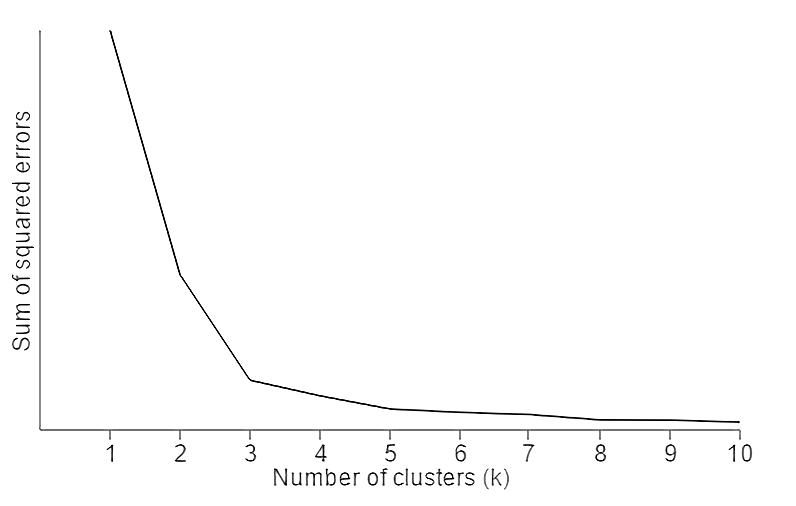
\includegraphics[width=0.8\textwidth]{res/elbow.png}
	\caption{Příklad grafu závislosti funkce J na počtu clusterů}
	\label{fig:obr1}
\end{figure}

Na obrázku \ref{fig:obr1} je na ose x počet shluků a na ose y výstup funkce J. V grafu hledáme místo, kde dochází k největšímu zlomu (zde ke zlomu dochází v případě 3 shluků). Metoda lokte není příliš spolehlivá u dat s velkým šumem, jelikož graf poměru počtu shluků a funkce J bude \uv{hladší} a nemůže tedy být spolehlivě řečeno, kdy zlom nastal. Metoda lokte musí být shora omezena maximálním počtem shluků, který musí být menší než celkový počet bodů v množině dat, jinak dojde k situaci, kdy se každému bodu přiřadí právě jeden shluk.

Metoda K-Medians je jedna z možných modifikací metody K-Means. Rozdíl spočívá v používání Manhattanské metriky pro přiřazování bodů k centroidům a výpočtu centroidů pomocí mediánu všech bodů shluku (po jednotlivých souřadnicích). Smysl modifikace spočívá v toleranci výchylek v datech.



\subsection{DBScan}
Principem algoritmu je nalezení nepřiřazeného bodu, kterým se začne tvořit nový shluk. Pokud se v \textepsilon okolí tohoto bodu nachází další body, jsou přidány do vznikajícího shluku a na všechny nově přidané je znovu aplikováno hledání dalších sousedů. Takto algoritmus najde $x$ bodů, které jsou od sebe vzájemně vzdálené maximálně \textepsilon. Pokud je $x$ větší než zvolené minimum, je shluk uznán za platný, v opačném případě je shluku rozpuštěn a pokračuje se dalším nepřiřazeným bodem. Jinými slovy -- hledají se pouze shluky od určitého počtu bodů. Algoritmus lze zapsat následovně:

\begin{enumerate}
	\item V množině bodů se najde první bod, který není přiřazen žádnému shluku a který ještě nebyl zvolen jako počáteční.
	\item Prohledá se \textepsilon okolí tohoto bodu a je-li nalezen další bod, je přidán do shluku
	\item Pro každý nově přidaný bod do shluku se provede krok (2) dokud budou další body přibývat. Není-li přidán žádný nový bod pokračuje se na krok (4)
	\item Pokud je v nově vzniklém shluku více bodů než je zadané minimum, je shluk uznán za platný, v opačném případě je rozpuštěn a pokračuje se novým počátečním bodem.
\end{enumerate}

DBScan, na rozdíl od metody K-Means, dokáže shluky určit i když nejsou lineárně oddělitelné (viz obrázek \ref{fig:obr2}) a navíc dokáže rozpoznat body, které jsou pouze šum (tzv. \textit{outliery}). DBScan také sám určuje počet shluků a není potřeba počet zadávat nebo vypočítávat.

\begin{figure}[h]
	\centering
	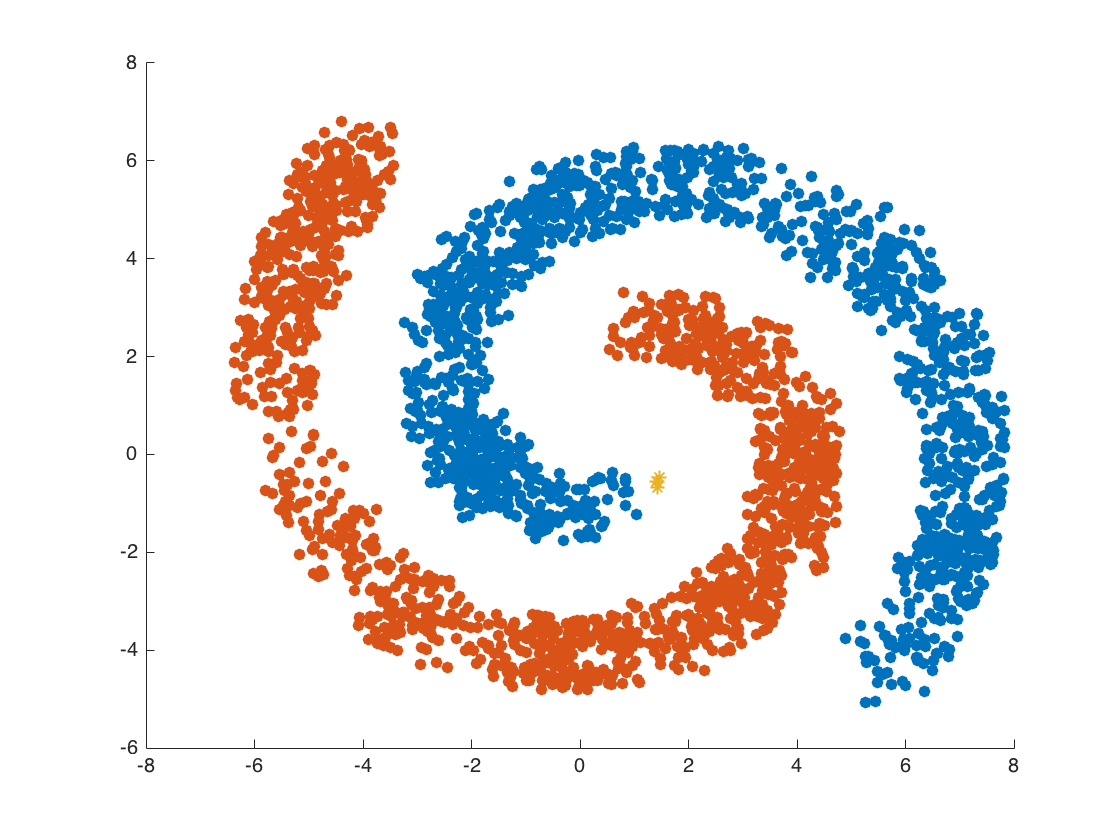
\includegraphics[width=0.8\textwidth]{res/dbscan.png}
	\caption{Lineárně neoddělitelné shluky nalezené algoritmem DBScan}
	\label{fig:obr2}
\end{figure}

\vspace{\baselineskip}

Pro svůj běh potřebuje znát dva parametry. Jejich volba vyžaduje určitou znalost dat.

\begin{enumerate}
	\item Minimální počet bodů, které smí utvořit shluk.
	\item Maximální vzdálenost dvou bodů \textepsilon. Body blíže než \textepsilon{} jsou považovány za sousedy.
\end{enumerate}




\newpage

\section{Popis implementace}
Aplikace byla naprogramována v jazyce Java ve verzi 8. Pro vytvoření grafického rozhraní byl použit designer obsažený v IDE JetBrains IntelliJ IDEA 2016. Při běhu jsou vypisovány na standardní výstup informace z průběhu shlukování.



\subsection{Implementovaná funkcionalita}
\noindent
Aplikaci lze rozdělit do dvou oddělených částí -- získání dat a zpracování dat.\\\\
\noindent
Pro získání dat byly implementovány následující 3 možnosti:
\begin{enumerate}
	
	\item Náhodný generátor uniformních dat (rovnoměrně umístěných po prostoru). Výstup představuje nejhorší možný scénář pro provedení shlukování, neboť se v datech nevyskytuje žádný přirozený shluk. Za shluk lze považovat pouze data jako celek.
	\begin{center}
		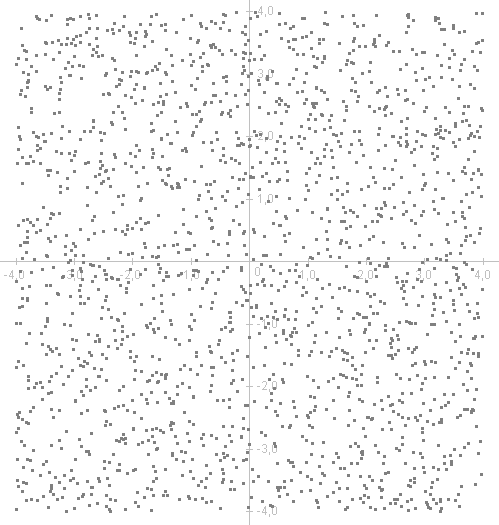
\includegraphics[width=0.5\textwidth]{res/datauniform.png}
	\end{center}

	\newpage

	\item Náhodný generátor shlukovaných dat. Výstup představuje (v optimálním případě) nejlepší možný scénář pro shlukování -- v datech se vyskytují jednoznačně oddělitelné shluky.
	\begin{center}
		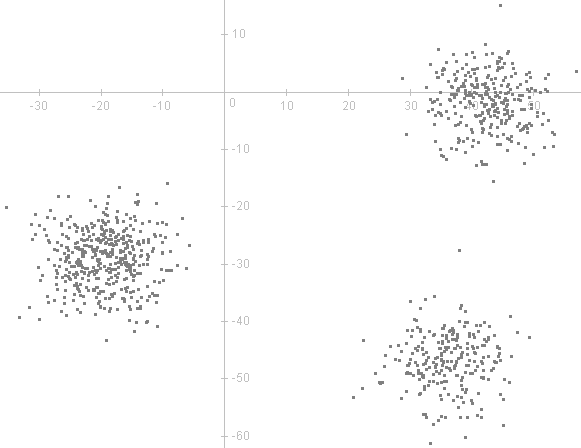
\includegraphics[width=0.5\textwidth]{res/dataclustered.png}
	\end{center}

	\item Načtení dat z externího souboru.
\end{enumerate}

\noindent
Zpracování dat, v případě této aplikace tedy provedení shlukování, bylo implementováno algoritmy K-Means, DBScan a K-Medians.

Bližší popis jednotlivých částí a jejich možností lze najít v kapitole \ref{subsec:prace-s-aplikace}.



\subsection{Rozdělení kódu}
Kód aplikace byl rozdělen dle vzoru MVC (model-view-controller), grafické rozhraní je tedy odděleno od aplikační/datové logiky. Jednotlivé části aplikace jsou odděleny do samostatných tříd s využitím technik OOP. Zde uvádíme pouze krátkých popis jednotlivých balíčků/tříd, konkrétnější informace jsou součástí kódové dokumentace (součást zdrojových kódu v javadoc formátu).

\begin{itemize}
	\item Třída \texttt{App} - obsahuje vstupní bod aplikace (\uv{main}), spouští aplikaci se standardním grafickým rozhraním.
	
	\item Třída \texttt{AppDev} - spouští aplikaci v režimu vhodném pro rychlé ladění/porovnání různých shlukovacích algoritmů nad shodnými daty. Ve výchozím stavu se pokouší načíst data ze souboru data.txt, v případě neúspěchu vygeneruje nová shlukovaná data a zpětně je uloží do zmíněného souboru.
\end{itemize}

\medskip

\begin{itemize}
	\item Třída \texttt{utils.ClusteringCanvas} - nástroj pro vygenerování grafu s daty. Používá se jako panel v rámci grafického rozhraní a též pro tvorbu grafu při exportu do externího souboru.
	
	\item Třída \texttt{utils.CsvDataProcessor} - obsahuje metody pro načtení/uložení dat z/do CSV souboru.
	
	\item Třída \texttt{utils.DataGenerator} - obsahuje metody pro generování náhodných dat.
	
	\item Rozhraní \texttt{utils.GUIController} - definuje rozhraní, pomocí kterého grafické rozhraní předává pokyny aplikační části.
	
	\item Třída \texttt{utils.GUIForm} - obsahuje samotné grafické rozhraní.
\end{itemize}

\medskip

\begin{itemize}
	\item Třída \texttt{structures.Point} - představuje instanci jednoho bodu libovolné dimenze. Obsahuje pomocné vlastnosti pro algoritmy a metody (například pro výpočet vzdálenosti od jiného bodu).
	
	\item Třída \texttt{structures.Cluster} - představuje shluk bodů (tedy instancí třídy Point). Je odděděno od třídy HashSet. Obsahuje metody pro operace nad shlukem (např. zjištění geometrického středu).
	
	\item Rozhraní \texttt{structures.ClusteringAlg} - definuje jednoduché rozhraní společné pro všechny shlukovací algoritmy.
	
	\item Rozhraní \texttt{structures.ClusteringAlgConf} - značkovací rozhraní tříd obsahujících konfigurace pro jednotlivé shlukovací algoritmy.
\end{itemize}

\medskip

\begin{itemize}
	\item Třídy \texttt{kmeans.KMeans}, \texttt{kmeans.KMeansConf} - třída provádějící shlukování algoritmem K-Means a třída s parametry pro provedení shlukování (tj. konfigurací).
	
	\item Třída \texttt{kmeans.KMedians} - odděděna od třídy KMeans, provádí shlukování algoritmem K-Medians.
	
	\item Třídy \texttt{dbscan.DBScan}, \texttt{dbscan.DBScanConf} - třída provádějící shlukování algoritmem DBScan a třída s parametry pro provedení shlukování (tj. konfigurací).
\end{itemize}


\newpage

\section{Uživatelská příručka}

\subsection{Překlad aplikace}
Překlad aplikace je možný nástrojem Ant, pomocí souboru build.xml v kořenovém adresáři. K překladu jsou nutné knihovny IDE IntelliJ IDEA (pro překlad GUI). Alternativně lze aplikaci přeložit po načtení projektu do zmíněného IDE.


\subsection{Spuštění aplikace}
Aplikaci lze spustit příkazem:
\\[2mm]
\texttt{\ldots\char`\\ > java -jar KMeans.jar}


\subsection{Práce s aplikací}\label{subsec:prace-s-aplikace}
Po spuštění se zobrazí grafické rozhraní, které se skládá z kontrolního panelu v levé části a oblasti pro vykreslení grafu v pravé části.


\begin{figure}[h]
	\centering
	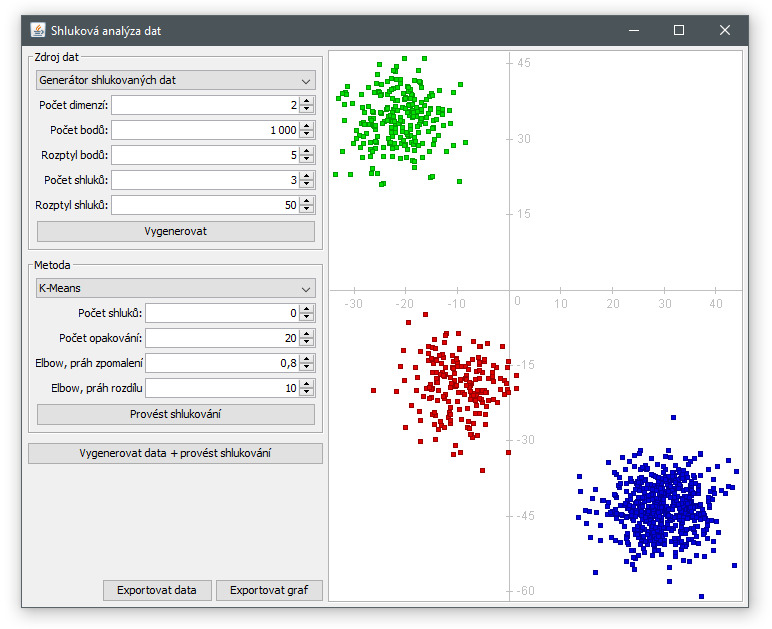
\includegraphics[width=1\textwidth]{res/gui.png}
	\caption{Grafické rozhraní aplikace}
	\label{fig:obr-gui}
\end{figure}


Kontrolní panel obsahuje dva základní bloky pro ovládání aplikace.

\subsubsection*{Zdroj dat}
Zde je možné vybrat metodu, která se použije pro generování náhodný dat, případně zvolit externí CSV soubor, ze kterého budou data načtena. V panelu je možné dle aktuálně zvolené možnosti nastavit různé parametry. Po stisknutí tlačítka jsou data vygenerována/načtena a okamžitě zobrazena v grafu.

\subsubsection*{Metoda}
Výběr jednoho ze tří implementovaných algoritmů, který bude použit pro provedení shlukování. Obdobně i zde je možné pro každou metodu nastavit různé parametry. Stisknutím tlačítka je poté shlukování zahájeno a výsledek zobrazen v grafu.

\begin{itemize}
	\item Metoda K-Means - výchozí algoritmus. Je možné nastavit počet shluků a počet opakování jednotlivých iterací algoritmu - pro výstup je vybrána iterace s nejlepším (tj. nejmenším) ohodnocením. V případě, že je počet shluků nastaven na nulu, je pro nalezení optimálního počtu shluků použita metoda lokte. Současně s tím se zpřístupní dva parametry pro nastavení této metody. Jejich popis se zobrazí po najetí myší nad příslušná pole.
	
	\item Metoda DBScan. Jako parametry lze nastavit minimální počet bodů v sousedství pro vytvoření shluku a maximální vzdálenost pro přidání sousedním bodů do shluku.
	
	\item Metoda K-Medians. Jedná se pouze o modifikaci metody K-Means, používá tedy i shodné nastavení.
\end{itemize}

Kontrolní panel dále obsahuje tlačítko, které provede obě zmíněné činnosti během jednoho kroku - tedy vygenerování/načtení nových dat a následně shlukování, obojí dle aktuálně nastavených parametrů. Ve spodní části panelu se dále nachází dvě tlačítka sloužící pro export - první z nich exportuje data do CSV souboru, druhý exportuje graf jako obrázek do souboru ve formátu PNG.


\subsubsection*{Import/export dat}
Aplikace umožňuje načíst data z externího souboru a rovněž data po shlukování exportovat. Pro tyto potřeby se používá jednoduchý tabulkový formát CSV, ve kterém je každý bod uložen na novém řádku, přičemž v jednotlivých buňkách (sloupcích) jsou souřadnice bodu (tedy každá \uv{osa} v novém sloupci). Jakmile se při načítání souřadnic narazí na nečíselnou hodnotu (tedy i prázdnou buňku), je zbytek řádku přeskočen. Očekává se, že všechny body budou mít stejný počet souřadnic; ten je zjištěn z prvního úspěšně načteného bodu. Soubor může mít například tuto podobu:

\begin{lstlisting}
1;1;1;;%*První bod*)
2;2;2;;%*Druhý bod*)
-2.164;3.14;21.66666;;%*Třetí bod*)
\end{lstlisting}


Při exportování dat je za souřadnice bodů vložen prázdný sloupec a poté sloupec s označením shluku:

\begin{lstlisting}
1;1;1;;Cluster 1
2;2;2;;Cluster 1
-2.164;3.14;21.66666;;Cluster 2
\end{lstlisting}



\section{Závěr}

Zadání bylo splněno v celém rozsahu. Vytvořená aplikace úspěšně demonstruje fungování vybraných shlukovacích algoritmů a umožňuje uživateli snadno vyzkoušet různé situace. Kód byl strukturován tak, aby bylo možné oddělit algoritmy od grafického rozhraní a použít samostatně. Aplikaci je možné snadno rozšířit o další funkcionalitu.

\end{document}


